\documentclass[a4paper,11pt]{article}	%classe e struttura

\usepackage[english]{babel} 	%lingua principale
\usepackage[utf8]{inputenc}	%caratteri accentati
\usepackage[margin=1in]{geometry}
%\usepackage{layaureo}

\usepackage{braket}
%\usepackage{physics}

\usepackage{graphicx}		%pacchetto per le immagini
\usepackage{booktabs}		%pacchetto per separatori tabelle
\usepackage{siunitx}		%pacchetto per le tabelle dati
\usepackage{wrapfig}		%pacchetto per le immagini immerse nel testo
\usepackage{latexsym}		%pacchetto per lettere greche
\usepackage[T1]{fontenc}
\usepackage{bm}
\usepackage{tabularx}
\usepackage{amsmath,amssymb,dsfont}
%\usepackage{bbold}

\usepackage{amsthm}
\usepackage{amsfonts}
\usepackage{subfig}
\usepackage{rotating}



\usepackage{tikz}
\usetikzlibrary{calc}
\usepackage{pgfplots}
\usepackage{tikz-3dplot}

%\linespread{2}



%\usepackage{fancyhdr}
\usepackage{hyperref}
%\pagestyle{fancy}
%\lhead{Rubens Longhi}
%\chead{}
%\rhead{A.A. 2015-2016}
%\lfoot{}
%\cfoot{\thepage}
%\rfoot{}
%\renewcommand{\headrulewidth}{0.4pt}
%\renewcommand{\footrulewidth}{0.4pt}
%%%%%%%%%%%%%%%%%%%%%%%%%%%%%%%%%%%%%%%%%%%%%%%%%%%%%%%%%%%%%%%%%%%%%%%%%%%%%%%%%%%%%%%%%%%
\newtheoremstyle{classicthm}% Nome
{12pt}% Spazio che precede l’enunciato
{12pt}% Spazio che segue l’enunciato
{\sl}% Stile del font dell’enunciato
{}% Rientro (se vuoto, non c’è rientro,
% \parindent = rientro dei capoversi)
{\bfseries}% Stile del font dell’intestazione
{.}% Punteggiatura che segue l’intestazione
{.5em}% Spazio che segue l’intestazione:
% " " = normale spazio inter-parola;
% \newline = a capo
{}% Specifica l’intestazione dell’enunciato
% (normalmente viene lasciata vuota)






\swapnumbers
\theoremstyle{classicthm}
\newtheorem{theorem}{Theorem}[section]
\newtheorem{theorem*}{Theorem}
\newtheorem{*theorem}[theorem]{$^*$Teorema}
\newtheorem{cor}[theorem]{Corollario}
\newtheorem{*cor}[theorem]{$^*$Corollario}
\newtheorem{**cor}[theorem]{$^{**}$Corollario}
\newtheorem{lem}[theorem]{Lemma}
\newtheorem{*lem}[theorem]{$^*$Lemma}
\newtheorem{prop}[theorem]{Proposition}
\newtheorem{*prop}[theorem]{$^*$Proposizione}
\newtheorem{**prop}[theorem]{$^{**}$Proposizione}
\newtheorem{axiom}[theorem]{Assioma}
\newtheorem{axiom*}{Assioma}

\theoremstyle{definition}
\newtheorem{defn}[theorem]{Definition}
\newtheorem{*defn}[theorem]{$^*$Definition}
\newtheorem{property}[theorem]{Propriet\`a}

\newtheorem{notation*}{Notazione}
\newtheorem{notation}[theorem]{Notazione}
%\newtheorem{Postulato}{Postulato}






\theoremstyle{definition}
\newtheorem{oss}[theorem]{Remark}
\newtheorem{exercise}[theorem]{Exercise}
\newenvironment{esercizio}{\begin{exercise}}{\hfill\medskip \end{exercise}}
\newenvironment{esercizio*}{\begin{exercise}}{\medskip\end{exercise}}
\newenvironment{commento}{\begin{oss}}{\endproof \end{oss}}
\newtheorem{*oss}[theorem]{$^*$Osservazione}
\newenvironment{*commento}{\begin{*oss}}{\endproof \end{*oss}}
\newenvironment{commento*}{\begin{oss}}{ \end{oss}}
\newtheorem{example}[theorem]{Example}
\newenvironment{esempio}{\begin{example}}{
	\end{example}}
	\newtheorem{*example}[theorem]{$^*$Esempio}
	\newenvironment{*esempio}{\begin{*example}}{\endproof	\end{example}}
	
	
	%\hypersetup{backref,pdfpagemode=FullScreen, colorlinks=true}
	
	\newcommand\ds{\displaystyle}
	\newcommand\ts{\textstyle}
	\newcommand{\mb}{\mathbf}
	%\renewcommand{\thenotation}{}
	%\renewcommand{\theequation}{\thesection.\arabic{equation}}
	\def\Caption #1{\caption{\footnotesize #1}}
	%\renewcommand\Caption{#1}{\Caption{\small{#1}}}
	%\def\Caption #1{\Caption{\small{{#1}}}}
	
	\def \Bfemph #1{\textbf{\emph{#1}}}
	
	
	%\def\Proof.{{\medbreak\noindent{\it Dimostrazione}\enspace}}
	\def\Proof{{\medbreak\noindent{\textbf{Proof.} }}}
	\def\endproof{~\hfill $\Box$\\}
	%\def\endproof{\hfill$\square$\par\medskip}
	
	\def\Svolgimento{{\medbreak\noindent{\textit{Svolgimento.} }}}
	\def\Suggerimento{{\medbreak\noindent{\textit{Suggerimento:} }}}
	
	
	
	
	
	\def\mR{{\mathbb R}}
	\def\mC{{\mathbb C}}
	\newcommand{\parz}[2]{\displaystyle \frac{\partial #1}{\partial #2}}
	\newcommand{\deri}[2]{\displaystyle \frac{d #1}{d #2}}
	\renewcommand{\Re}{\operatorname{Re}}
	\renewcommand{\Im}{\operatorname{Im}}
	%\renewcommand{\theta}{\vartheta}
	\newcommand{\Int}{\text{Int }}
	\newcommand{\Ext}{\text{Ext }}
	\newcommand{\supp}{\text{supp}}
	\newcommand{\mD}{\mathcal{D}}
	\newcommand{\dd}{\mathrm d}
	\newcommand{\norm}[1]{\displaystyle \left \| #1 \right \|}
	\newcommand{\abs}[1]{\displaystyle \left | #1 \right |}
	\renewcommand{\div}{\operatorname{div}}
	\newcommand{\id}{\mathds{1}}
	\newcommand{\supc}[1]{C_0^\infty(#1)}
	\newcommand{\mf}[1]{\mathbf{#1}}
	
	
	\def\Xint#1{\mathchoice 
		{\XXint\displaystyle\textstyle{#1}}% 
		{\XXint\textstyle\scriptstyle{#1}}% 
		{\XXint\scriptstyle\scriptscriptstyle{#1}}% 
		{\XXint\scriptscriptstyle\scriptscriptstyle{#1}}% 
		\!\int} 
	\def\XXint#1#2#3{{\setbox0=\hbox{$#1{#2#3}{\int}$} 
			\vcenter{\hbox{$#2#3$}}\kern-.5\wd0}} 
	\def\Mint{\Xint -}
	
	
	\renewcommand{\hat}[1]{\widehat{#1}}
	\renewcommand{\theta}{\vartheta}
	\let\oldepsilon\epsilon
	\renewcommand{\epsilon}{\varepsilon}
	\renewcommand{\phi}{\varphi}
	\newcommand{\res}{\mathop{\mathrm{Res }}}
	
	\newcommand{\colonna}[2]{\begin{pmatrix}
			#1 \\ #2
		\end{pmatrix}}
		\newcommand{\riga}[2]{\begin{pmatrix}
				#1 & #2
			\end{pmatrix}}
			%%%%%%%%%%%%%%%%%%%%%%%%%%%%%%%%%%%%%%%%%%%%%%%%%%%%%%%%%%%%%%%%%%%%%%%%%%%%%%%%%%%%%%%%%%%
			
			
			
			\frenchspacing 		%regola spazi
			\raggedbottom		%spazio vuoto a fine pagina, quando finisce il testo

\title{Introduction to Green functions}
\author{Rubens Longhi}
\date{November 8, 2017}


\begin{document}
%\begin{huge}
\maketitle		%crea titolo
%\tableofcontents
%\newpage
\section{Resolvent}

The general solution of a linear differential equation in the form
\[	L\psi=f	\]
is given by the sum of a generic solution $u_0$ to the homogeneous equation $Lu_0=0$ and a particular solution $u$:
\[	\psi(x)=u_0(x)+u(x).	\]
The aim is to build a way to provide a particular solution to any non-homogeneous differential equation with a source $f$, in fact we will need do invert the operator $L$ in such a way that holds
\[	u=L^{-1}f.	\]
The method described relies on the determination of a function, called \emph{Green function}, which allows to find the solution of a differential equation regardless the specific form of the source.

\begin{defn}
	Let $\Omega$ be an open subset\footnote{if $n=1$, $\Omega$ can be a closed subset, because we can define the derivatives at the border points.} of $\mR^n$, let $ L=\sum_{\alpha}c_\alpha\partial^\alpha$ be a linear differential operator with a multi-index $\alpha\in\mathbb{N}^n$.\\ An operator $\mathds{G}:C_0^\infty(\Omega)\to C^\infty(\Omega)$ is called \emph{Green operator} or \emph{resolvent} for $L$ if $\mathds{G}=L^{-1}$ is an inverse of $L$,
	\[	L\mathds{G}=\mathds{G}L|_ {\supc{\Omega}}=\mathds{1}.		\]
\end{defn}

\noindent Notice that the request $L\mathds{G}f=f$ for any $f\in\supc{\Omega}$ means that $u=\mathds{G}f$ is a solution to the differential equation
\[	Lu=f.	\]
Conversely, the request $\mathds{G}Lu=u$ for any $u\in C^\infty(\Omega)$ means that $u$ must be the solution of the problem when $f$ is chosen to be $Lu$.\\

\noindent If $L$ is a differential operator, one expects that the inverse must have the form of an integral operator. Hence the following:

\begin{defn}
	Let $\mathds{G}$ be a Green operator for $L$. A function $G\in\operatorname{L}^1(\Omega\times\Omega)$ is a \emph{Green function} for $L$ if for all $f\in \supc{\Omega}$ holds
	\[	(\mathds{G}f)(x)=\int_\Omega G(x,y)f(y)\,\dd y, \quad\forall x\in\Omega. 	\]
	For fixed $y\in\Omega$, the function $x\mapsto G(x,y)$ is called \emph{fundamental solution} for $L$ at $y$.
\end{defn}

\noindent Notice that in this case $\mathds{G}$ is an integral operator with kernel $G$.\\

\noindent Given any source $f$, a particular solution of $Lu=f$ can be written in the form
\begin{equation}
		u(x)=	\int_\Omega G(x,y)f(y)\,\dd y.	\label{soluzione}
\end{equation}

\begin{prop}
	$G$ is a Green function for the differential operator $L$ if and only if holds:
	\begin{itemize}
		\item $L_xG(x,y)=\delta(x-y)$,
	\end{itemize}
	where $L_x$ denotes that $L$ acts only on the $x$ variable and the derivatives are intended in distributional sense.
\end{prop}
\Proof Applying $L$ to the solution in equation \eqref{soluzione}, for any $f$ holds
\[	f(x)=Lu(x)=\int_\Omega L_xG(x,y)f(y)\,\dd y.	\]
The only way the formula holds is if $L_xG(x,y)=\delta(x-y)$.
\endproof


\begin{oss}
	If we find two independent Green functions $G_1,G_2$, then it is easy to find a solution to the homogeneous equation $Lu=0$: in fact, if $u(x)=\int (G_1-G_2)(f)$, then $Lu=\delta-\delta=0$.
\end{oss}

\begin{esempio}[Waves on a string]
	Let $\Omega=[0,\infty)\times[0,l]$, the variable is $(t,x)$ and $L=\partial_x^2-\partial_t^2$. The equation
	\[	(\partial_x^2-\partial_t^2)\psi(t,x)=0	\]
	is called the homogeneous \emph{wave equation}. Now we use the method of separation of variables: let the solution be of the form $\psi(t,x)=u(x)e^{-ikt}$. Differentiating we obtain
	\[	u''(x)+k^2u(x)=0.		\]
	If now we introduce a perturbation $f(x)$ distributed along $[0,l]$, the equation becomes
	\begin{equation}
		u''(x)+k^2u(x)=f(x).
		\label{eq:forcedoscillator}
	\end{equation}
	We look for solutions $u$ with the constraints
	\[	u(0)=u(l)=0.		\]
	We assume a generic solution of the form
	\[	u(x)=A(x)\cos kx+B(x)\sin kx, 		\]
	in this case there are some constraints on the derivatives that we will require in order to find a particular solution more easily:
	\begin{equation}
		A'(x)\cos kx+B'(x)\sin kx=0.
		\label{eq:constr}
	\end{equation}
	Differentiating, we have
	\[	u'(x)=A'(x)\cos kx -kA(x)\sin kx+B'(x)\sin kx+kB(x)\cos kx,		\]
	and making use of Equation \eqref{eq:constr},
	\[	u''(x)=k\left[B'(x)\cos kx-k B(x)\sin kx -A'(x)\sin kx-k A(x)\cos kx \right].		\]
	The differential equation \eqref{eq:forcedoscillator} becomes
	\[	-kA'(x)\sin kx +k B'(x)\cos kx=f(x).		\]
	Combining last equation with \eqref{eq:constr}, we obtain
	\[	A'(x)=-\frac1k	f(x)\sin kx,\qquad B'(x)=\frac1k f(x)\cos kx,	\]
	\[	A(x)=-\frac1k \int_{c_1}^{x}f(y)\sin ky\,\dd y,\qquad B(x)=\frac1k\int_{c_2}^{x} f(y)\cos ky	\,\dd y.		\]
	Then the solution becomes
	\[	u(x)=-\frac1k \cos kx\int_{c_1}^{x}f(y)\sin ky\,\dd y+\frac1k \sin kx \int_{c_2}^{x} f(y)\cos ky	\,\dd y.			\] 
	The constraint $u(0)=0$ implies
	\[	0=-\frac1k\int_{c_1}^{0}f(y)\sin ky\,\dd y,		\]
	from which we obtain $c_1=0$.
	The constraint $u(l)=0$ implies
	\[	-\frac1k \cos kl\int_{0}^{l}f(y)\sin ky\,\dd y+\frac1k \sin kl \int_{c_2}^{l} f(y)\cos ky	\,\dd y	=0.		\]
	Now, from $\int_{c_2}^{l}=\int_{c_2}^{0}+\int_{0}^{l}$, it holds
	\[	\frac1k\int_{0}^{l}\left[-\cos kl\sin ky+\sin kl\cos ky\right]f(y)\,\dd y+\frac1k\sin kl\int_{c_2}^{0}f(y)\cos ky\,\dd y=0,		\]
	\[	\frac1k\int_{0}^{l}\sin  k(l-y)\,f(y)\,\dd y+\frac1k\sin kl\int_{c_2}^{0}f(y)\cos ky\,\dd y=0,		\]
	\[	\frac1k\int_{c_2}^{0}f(y)\cos ky\,\dd y=-\frac1{k\sin kl}\int_{0}^{l}\sin  k(l-y)\,f(y)\,\dd y.		\]
	Now, from $\int_{c_2}^{x}=\int_{c_2}^{0}+\int_{0}^{x}$, it holds
	\[	u(x)=-\frac1k \int_{0}^{x}f(y)\left[\cos kx\sin ky-\sin kx\cos ky\right]\,\dd y-\frac{\sin kx}{k\sin kl}\int_{0}^{l}\sin  k(l-y)\,f(y)\,\dd y,	\]
	\[	u(x)=\frac1k \int_{0}^{x}f(y)\sin k(x-y)\,\dd y+\frac{\sin kx}{k\sin kl}\int_{0}^{l}\sin  k(y-l)\,f(y)\,\dd y,		\]
	Now, from $\int_{0}^{l}=\int_{0}^{x}+\int_{x}^{l}$, holds
	\[	u(x)=\frac1k \int_{0}^{x}f(y)\left[\frac{\sin kl\sin k(x-y)+\sin kx\sin k(y-l)}{\sin kl}\right]\,\dd y+\frac{\sin kx}{k\sin kl}\int_{x}^{l}\sin  k(y-l)\,f(y)\,\dd y.	\]
	One can easily check $$\sin kl\sin k(x-y)+\sin kx\sin k(y-l)=\sin ky\sin k(x-l),$$ and one has
	\begin{equation}
			u(x)=	\int_0^l G(x,y)f(y)\,\dd y,
	\end{equation}
	with
	\[	G(x,y)=\begin{cases}
	\dfrac{\sin ky\sin k(x-l)}{k\sin kl}\quad& y\in[0,x]\\
	\\
	\dfrac{\sin kx\sin k(y-l)}{k\sin kl}\quad& y\in[x,l].
	\end{cases}		\]
	One can notice that the Green function is symmetric: $$G(x,y)=G(y,x),$$ that $$G(x,0)=G(x,l)=0,$$ and that $G$ is continuous and differentiable excepts when $x=y$, in fact
	\[	\lim_{y\to x^+}\parz{G}{y}(x,y)-\lim_{y\to x^-}\parz{G}{y}(x,y)=1.	\]
	Now we can verify $\partial_x^2G(x,y)+k^2G(x,y)=\delta(x-y)$.\\
	One can easily compute $\partial_x^2G(x,y)+k^2G(x,y)=0$ for $x\neq y$, then in general holds:
	\[	u(y)=\int_{0}^{l}f(x)G(x,y)\,\dd x=\int_{0}^{l}\left[u''(x)+k^2u(x)\right]G(x,y)\,\dd x,		\]
	and integrating two times by parts and throwing away the border terms:
	\[	u(y)=\int_{0}^{l}f(x)G(x,y)\,\dd x=\int_{0}^{l}\left[\partial_x^2 G(x,y)+k^2G(x,y)\right]u(x)\,\dd x,		\]
	and then it follows the result.\\
	The equation $\partial_x^2G(x,y)+k^2G(x,y)=\delta(x-y)$ can be interpreted as the differential equation for the displacement from the equilibrium position provoked by an impulse concentrated at $y$. The solution $u(x)$ is the superposition of all the displacements in $x$ provoked by $f(y)$ and distributed all along the string.
\end{esempio}

\section{Fundamental solutions and Fourier transform}

	There may be the case of a global translational symmetry for the differential equation (i.e. there are no finite boundary conditions and taking the derivatives at some point is the same as taking them at any other point), in which the Green function depends only from the displacement: $G(x,y)=\widetilde{G}(x-y)$. In this case we will often denote, with abuse of notation  $G(x-y)=\widetilde{G}(x-y)$. It is clear that holds
	\begin{equation}
	u(x)=\int_{\mR^n} G(x-y)f(y)\,\dd y=(G*f)(x),\label{eq:convolution}
	\end{equation}
	where $*$ stands for the convolution.\\
	In case of symmetry, it suffices to find a fundamental solution at a fixed point, for example $y=0$, $G(x,0)$ and the problem is solved globally by convolution.

\begin{theorem}
	\label{theorem:1}
	Let $L:C^\infty(\mR)\to C^\infty(\mR)$ such that $L=\sum_k c_k\partial_t^k$ is a linear differential operator with constant coefficients. Let $P(s)=\sum_k c_k s^k$ be the characteristic polynomial associated with $L$.\\ A fundamental solution $G$ for $L$ at $t=0$ (i.e. a solution of $LG(t)=\delta(t)$) is given by the \emph{Fourier transform} of $1/P(-i\omega)$, in other words holds the formula
	\begin{equation}
	G(t)=\frac{1}{2\pi}\int_{-\infty}^{+\infty} G(\omega)e^{-i\omega t}\,\dd\omega, \text{ where }\ G(\omega)=\frac1{P(-i\omega)}.
	\label{eq:solfou}
	\end{equation}
\end{theorem}
\Proof Write $G(t)$ in terms of its inverse Fourier transform:
\[	G(t):=\frac1{2\pi}\int_{-\infty}^{+\infty}G(\omega)e^{-i\omega t}\,\dd\omega,		\]
and put it into $LG=\delta$. One obtains
\[	\frac1{2\pi}\int_{-\infty}^{+\infty}P(-i\omega) G(\omega)e^{-i\omega t}\,\dd\omega=\frac1{2\pi}\int_{-\infty}^{+\infty}e^{-i\omega t}\,\dd\omega,		\]
where we used the fact that $Le^{st}=P(s)e^{st}$ and holds
\[	\delta(t)=\frac1{2\pi}\int_{-\infty}^{+\infty}e^{-i\omega t}\,\dd\omega.		\]
Now, the integrand must be equal side-by-side, hence we have
\[	P(-i\omega)G(\omega)=1.			\]
Then the thesis holds.
\endproof

\begin{oss}
	In equation \eqref{eq:solfou} we can make the substitution $y=-i\omega$. The differential becomes $\dd y=-i\dd\omega$ and the integral becomes
	\[G(t)=\frac{1}{2\pi i}\int_{-i\infty}^{+i\infty}\frac{e^{y t}}{P(y)}\,\dd y,\]
	which is the \emph{inverse Laplace transform} of $1/P(y)$.
\end{oss}

\begin{oss}
	The operator $L$ in Theorem \ref{theorem:1} is invariant under translations, so it suffices to find a fundamental solution at one point.
\end{oss}


\section{Driven harmonic oscillator with viscosity}

Now we want to find Green functions for the \emph{driven and damped harmonic oscillator}. If $x(t)$ is the displacement from the equilibrium position, $\gamma$ indicates the strength of the damping, $\omega_0$ is the proper angular frequency and we take into account a force $f(t)$, the equation has the form
\begin{equation}
	x''(t)+2\gamma x'(t)+\omega_0^2 x(t)=f(t).
	\label{eq:forceddamped}
\end{equation}
\subsection{No damping}

To start, we take into account the case in which $\gamma=0$. The solution when $f(t)=f_0e^{-i\omega t}$ is the sum of the general homogeneous solution
\[	x(t)=x_0e^{-i(\omega_0 t+\phi)},			\]
and a particular solution. If we try with $x(t)=A(\omega)e^{-i(\omega t+\alpha)}$, putting it in the equation we obtain \[\alpha=0\qquad A(\omega)=\frac1{\omega_0^2-\omega^2}f_0, \]
which results in phase with the force $f$.\\

\noindent We want now to solve for the fundamental solution at $t=0$: $G_0(t)$ such that
\[	G_0''(t)+\omega_0^2G_0(t)=\delta(t).		\]
The characteristic polynomial is $P(s)=s^2+\omega_0^2$, hence\footnote{notice that holds $G(\omega)=A(\omega)/{f_0}$ }
\begin{equation}
G_0(\omega)=\frac1{P(-i\omega)}=\frac1{\omega_0^2-\omega^2}.\label{eq:Gomegazero}
\end{equation}
The integral to calculate is that in equation \eqref{eq:solfou}:
\[G_0(t):=\frac1{2\pi}\int_{-\infty}^{+\infty}\frac{e^{-i\omega t}}{\omega_0^2-\omega^2}\,\dd\omega.\]
We will end up showing that
\[	G_0(t)=\Theta( t)\frac{\sin\omega_0t}{\omega_0},		\]
but there is a problem.\\

\noindent If we try to calculate the integral for $G_0(t)$ we encounter a problem: the function has two second-order poles on the real axis, hence it is not integrable!\\
In order to calculate the integral in the former expression we must introduce a regularization. The integral will become a limit of integrals calculated in such a way that the poles are slightly removed from the real axis.\\ One can show that there are two independent types of possible regularizations: one type is realized when the poles are shifted to the upper complex semi-plane, the other type is realized when the poles are shifted in the lower semi-plane. The latter regularization produces a function supported in the past and the former one produces a function supported in the future. They are often called respectively \textbf{retarded} and \textbf{advanced} fundamental solutions. We will chose the \emph{retarded} of regularization because we want to propagate the impulse generated at $t=0$.
\[	G_0(t)=\lim_{\epsilon\to0^+}G_\epsilon(t).	\]
We choose the regularization such that the function vanishes for $t<0$.
\[G_\epsilon(t):=\frac1{2\pi}\int_{-\infty}^{+\infty}\frac{e^{-i\omega t}}{\omega_0^2-\omega^2-2i\omega\epsilon}\,\dd\omega,\]
and we make use of techniques of complex analysis as follows.\\
\noindent Denote
\begin{itemize}
	\item $\ds\beta:=\sqrt{1-\left(\dfrac{\epsilon}{\omega_0}\right)^2}$, where $\beta\to1$ if $\epsilon\to 0$;
	\item $C_\rho^+$ the upper half-circle of radius $\rho$ centered at $\omega=0$ which has $\Im(\omega)>0$, oriented counter-clockwise;
	\item $C_\rho^-$ the lower half-circle of radius $\rho$ centered at $\omega=0$ which has $\Im(\omega)<0$, oriented clockwise;
	\item $[-\rho,\rho]$ the interval of the real line connecting $-\rho$ and $\rho$, oriented from left to right.
\end{itemize}
The singularities are
\[\omega_\pm=-i\epsilon\pm\sqrt{\omega_0^2-\epsilon^2}= -i\epsilon\pm\omega_0\beta.\]
\begin{figure}[h]
	\centering
	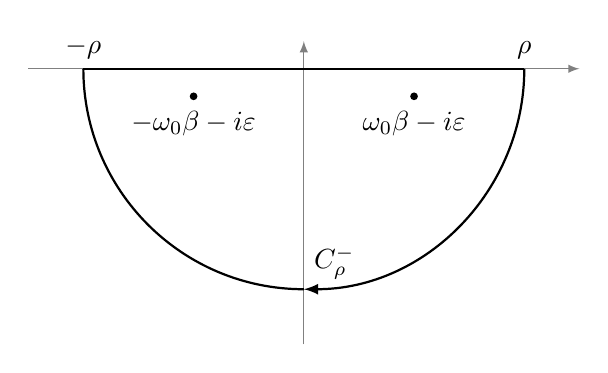
\begin{tikzpicture}[scale=0.7][>=latex]
	%\tikzstyle{every node}=[font=\scriptsize]
	\coordinate (Origin)   at (0,0);
	\coordinate (XAxisMin) at (-5,0);
	\coordinate (XAxisMax) at (5,0);
	\coordinate (YAxisMin) at (0,-5);
	\coordinate (YAxisMax) at (0,0.5);
	\draw [thin, gray,-latex] (XAxisMin) -- (XAxisMax) ;% Draw x axis
	\draw [thin, gray,-latex] (YAxisMin) -- (YAxisMax) ;% Draw y axis
	
	%\clip (-5,-5) rectangle (10cm,10cm); % Clips the picture...
	
	
	
	\draw [thick,-latex] (4cm,0mm) node[above] {$\rho$} arc [start angle=0, end angle=-90, radius=4cm] node[above right] {$C_\rho^-$};
	\draw [thick] (0,-4cm) arc [start angle=-90, end angle=-180, radius=4cm] node[above] {$-\rho$};
	\draw [thick] (-4,0) -- (4,0);
	
	\draw (-2,-0.6) node[below] {$-\omega_0\beta-i\epsilon$};
	\draw (2,-0.6) node[below] {$\omega_0\beta-i\epsilon$};
	\fill (-2,-0.5) circle (0.07);
	\fill (2,-0.5) circle (0.07);
	
	
	
	
	
	
	\end{tikzpicture}
	
	\caption{The circuit to compute $ G_\epsilon(t)$ for $t>0$.}	\label{fig:integrale2}
	
\end{figure}
Hence we have
\[\text{for } t<0\quad   G_\epsilon(t)=\frac1{2\pi}\lim_{\rho\to\infty}\int_{C_\rho^++[-\rho,\rho]}\frac{e^{-i\omega t}}{\omega_0^2-\omega^2-2i\epsilon\omega}\,\dd\omega=\frac1{2\pi}2\pi i\sum\operatorname{Res}=0,\]
where the sum is extended to the singularities in the upper half-plane. The expression vanishes because we choose the circuit such that the integral on $C_\rho^+$ vanishes in virtue of Jordan's lemma and there are no singularities in the region bounded by the circuit.\\
The non-zero integral is
\[	 G_\epsilon(t), \text{ for } t>0.	\] 
It is computed via the lower circuit in \textsc{Figure} (\ref{fig:integrale2}
): $C_\rho^-+[-\rho,\rho]$, in order to get rid of contributes from the half-circles.\\

\noindent The results are 
\[	\text{for } t>0\quad  G_\epsilon(t)=-\frac1{2\pi}2\pi i\sum_{\omega_\pm}\operatorname{Res}= ie^{-\epsilon t}\left(\frac{e^{-i\beta\omega_0t}-e^{i\beta\omega_0t}}{2\beta\omega_0}\right)= \frac{\sin\beta\omega_0t}{\beta\omega_0}e^{-\epsilon t},		\]
Summing up everything in one formula:
\begin{equation}
 G_\epsilon(t)= \Theta( t)\frac{\sin\beta\omega_0t}{\beta\omega_0}e^{-\epsilon t}=\Theta( t)\frac{\sin\sqrt{\omega_0^2-\epsilon^2}t}{\sqrt{\omega_0^2-\epsilon^2}}e^{-\epsilon t},
\label{eq:integralone}
\end{equation}
where $\Theta$ is the Heaviside step-function. Taking the limit, the result is
\begin{equation}
	G_0(t)=\lim_{\epsilon\to 0^+}G_\epsilon(t)=\Theta( t)\frac{\sin\omega_0t}{\omega_0}.
\end{equation}
The claim is that $G_0(t)$ is a fundamental solution for the forced oscillator at $0$. In fact, recalling that
\[	\Theta'(t)=\delta(t),\qquad	-t\delta'(t)=\delta(t),		\]
it holds
\[	G_0''(t)+\omega_0^2G_0(t)=\left(2\cos\omega_0 t-\frac{\sin\omega_0 t}{\omega_0 t}\right)\delta(t),		\]
but $\delta(t)=0$ if $t\neq 0$, so $G_0(t)$ is a fundamental solution:
\[	G_0''(t)+\omega_0^2G_0(t)=\delta(t).		\]
The function $G_0(t)$ is the response of the system to an impulsive solicitation at $t=0$.\\
Hence, the Green operator becomes, recalling equation \eqref{eq:convolution},
\[	x(t)=G_0(t)*f(t)=\int_{-\infty}^{\infty}G_0(t-t')\,f(t')\,\dd t'=\int_{-\infty}^{t}G_0(t-t')\,f(t')\,\dd t',		\]
where the integral stops at $t$ because of Heaviside step-function appearing in $G_0$.\\
This fact is expression of the physical principle of causality: the effects at time $t$ are the superposition of the events of the past.

\subsection{Driven harmonic oscillator}

Now we come back to equation \eqref{eq:forceddamped} in case $f(t)=f_0e^{-i\omega t}$. The solutions of the homogeneous equation are universally known:
\begin{equation}
	x(t)=e^{-\gamma t}\left[c_1e^{\alpha t}+c_2e^{-\alpha t}\right],
	\label{eq:homodriven}
\end{equation}		
with $\alpha=\sqrt{\gamma^2-\omega_0^2}$. If $\gamma>\omega_0$ the oscillator goes exponentially to the equilibrium. Otherwise, the system oscillates with an amplitude that decays exponentially.\\
To find a particular solution we try with
\[	x(t)=A(\omega)e^{-i\omega t}.		\]
Putting it into the equation, we obtain
\[	A(\omega)=\frac{f_0}{\omega_0^2-\omega^2-2i\gamma\omega}=f_0\frac{\omega_0^2-\omega^2+2i\omega\gamma}{(\omega_0^2-\omega^2)+4\omega^2\gamma^2}=f_0\rho e^{i\phi}.		\]
The module $\rho$ is
\[	\rho=\frac{1}{\sqrt{(\omega_0^2-\omega^2)^2+4\omega^2\gamma^2}},		\]
and the phase $\phi$ is such that $\tan \phi=\dfrac{\Im A}{\Re A}=\dfrac{2\gamma\omega}{\omega_0^2-\omega^2}$, hence the solution can be expressed as
\begin{equation}
	x(t)=\frac{1}{\sqrt{(\omega_0^2-\omega^2)^2+4\omega^2\gamma^2}}f_0e^{-i(\omega t-\phi)}.
	\label{eq:solutiongeneral}
\end{equation}
We want to find a fundamental solution $G(t)$ at $t=0$, in other words we want to solve:
\[	G''(t)+2\gamma G'(t)+\omega_0^2G(t)=\delta(t).		\]
Now, as before, we introduce the function $G(t)$ and its Fourier transform $G(\omega)$ and we transform the differential equation.\\
The characteristic polynomial is $P(s)=s^2+2\gamma s+\omega_0^2$, hence we have\footnote{notice that again it holds $G(\omega)=A(\omega)/{f_0}$ }
\[	G(\omega)=\frac1{P(-i\omega)}=\frac{1}{\omega_0^2-\omega^2-2i\gamma\omega},\qquad G(t)=\frac1{2\pi}\int_{-\infty}^{\infty}\frac{e^{-i\omega t}}{\omega_0^2-\omega^2-2i\gamma\omega}\,\dd\omega.		\]
The former integral is exactly the same computed in equation \eqref{eq:integralone}, with the substitution $\epsilon=\gamma$, so it holds
\[	G(t)=\Theta( t)\frac{\sin\beta\omega_0t}{\beta\omega_0}e^{-\gamma t}.	\]
This tells us that the damped oscillator admits only a \emph{retarded} fundamental solution and the operation of shifting the poles corresponds to the addition of a damping therm in the differential equation.\\
If the damping $\gamma$ is negligible with respect to  $\omega_0$, i.e. $\gamma\ll\omega_0$, then $\beta=\sqrt{1-(\frac{\gamma}{\omega_0})^2}$ rapidly converges to $1$, then we have
\begin{equation}
		G(t)=\Theta( t)\frac{\sin\omega_0t}{\omega_0}e^{-\gamma t}\quad\text{for }\gamma\ll\omega_0.
		\label{eq:greendamp}
\end{equation}
Again, equation \eqref{eq:greendamp} is a fundamental solution at $t=0$, if $\gamma\ll\omega_0$:
\[	G''(t)+2\gamma G'(t)+\omega_0^2G(t)=\delta(t).		\]
Hence, the Green operator becomes, recalling equation \eqref{eq:greendamp} and equation \eqref{eq:convolution},
\[	x(t)=G(t)*f(t)=\int_{-\infty}^{\infty}G(t-t')\,f(t')\,\dd t'=\int_{-\infty}^{t}G(t-t')\,f(t')\,\dd t',		\]
where the integral stops at $t$ because of Heaviside step-function appearing in $G$.\\
The function $G$ is the Green function of the system: it represents the response to a Dirac delta function input at $t=0$ that decades to zero with a lifetime $\gamma^{-1}$.

\subsection{Resonance}

In low damping regime, after a meantime of $\gamma^{-1}$, the homogeneous solution in Equation \eqref{eq:homodriven} becomes negligible, and the system goes on with the particular solution in equation \eqref{eq:solutiongeneral} with constant amplitude and with the same frequency of $f$. The \emph{transmitted} amplitude is maximum when the denominator in equation \eqref{eq:solutiongeneral} becomes minimum. With a simple derivative, one shows that maximum amplitude is at
\[	\omega^2=\omega_0^2-2\gamma^2,	\]
which is called \emph{resonance in amplitude}. For the velocity we have $$x'(t)=\frac{-i\omega}{\sqrt{(\omega_0^2-\omega^2)^2+4\omega^2\gamma^2}}f_0e^{-i(\omega t-\phi)}=\frac{\omega}{\sqrt{(\omega_0^2-\omega^2)^2+4\omega^2\gamma^2}}f_0e^{-i(\omega t-\phi+\frac{\pi}{2})},$$
hence the \emph{resonance in energy (or in velocity)} happens when
\[	\omega=\omega_0,	\]
and in this case $\tan\phi=\dfrac{2\gamma\omega}{\omega_0^2-\omega^2}\to \infty$, $\phi=\frac{\pi}{2}$, so, in resonance, the signal is in phase with the force $f$.\\

\noindent Let now define the function, called \emph{spectral density}
\begin{equation}
	S(\omega)=-\frac{1}{2\pi i}\left[G^*(\omega)-G(\omega)\right]=\frac{1}{\pi}\frac{\frac12\Gamma(\omega)}{(\omega_0^2-\omega^2)^2+\frac14\Gamma^2(\omega)},
\end{equation}

\begin{figure}[h]
	\centering
	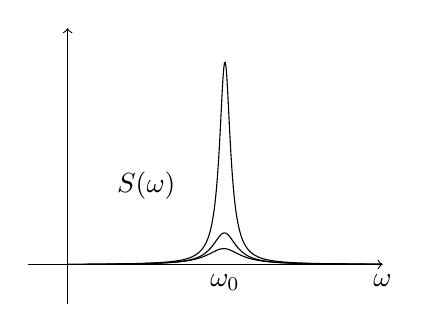
\begin{tikzpicture}[domain=0:4,samples=400]
	\draw[->] (-0.5,0) -- (4,0) node[below] {$\omega$};
	\draw[->] (0,-0.5) -- (0,3)% node[left] {$y$}
	;
	%\foreach \i in {50,100,...,200} {
	%	\draw (\i,1) -- (\i,-1) node[below] {$\i$};
	%	}
	%	\foreach \i in {10,20,...,40} {
	%	\draw (1,\i) -- (-1,\i) node[left] {$\i$};
	%	}

	\draw[black] plot[domain=0:2,samples=400] (2*\x,{(\x/56)/((1-\x*\x)*(1-\x*\x)+0.25*(\x*\x/36)});
	\draw[black] plot[domain=0:2,samples=400] (2*\x,{(\x/75)/((1-\x*\x)*(1-\x*\x)+0.5*(\x*\x/15)});
	\draw[black] plot[domain=0:2,samples=400] (2*\x,{(\x/75)/((1-\x*\x)*(1-\x*\x)+1*(\x*\x/15)});
	\node[below] at (2,0) {$\omega_0$};
	\node[fill=white,rounded corners=1pt,inner sep=0.5pt] at (1,1) {$S(\omega)$};
	%\draw[red] plot (\x,{5/\x});
	\end{tikzpicture}
	
\end{figure}
where $\Gamma(\omega)=4\omega\gamma$. $S(\omega)$ has a maximum when there is resonance in energy ($\omega=\omega_0$). $\Gamma(\omega)$ represents the width of the Lorentzian $S(\omega)$ and when $\gamma\ll\omega_0$, we can approximate the FWHM \noindent with $\Gamma(\omega_0)=4\omega_0\gamma$.
When the damping $\gamma$ goes to $0$, $S(\omega)$ converges to a Dirac delta $\delta(\omega-\omega_0)$.\\
The effect of the damping is that of transporting the poles of $G_0(\omega)$ out of the real axis as in $G(\omega)$, as we have seen before.\\ The link between $G(\omega)$ and $G_0(\omega)$ can be easily understood if one introduces the so-called \emph{self-energy} $$\Sigma^\star(\omega)=2i\omega\gamma,$$
\begin{equation}
	G(\omega)=\frac{1}{\omega_0^2-\omega^2-\Sigma^\star(\omega)}=\frac{1}{[G_0(\omega)]^{-1}-\Sigma^\star(\omega)}.
	\label{eq:Gresolved}
\end{equation}
$\Sigma^\star(\omega)$ represents the interaction between the oscillator and the environment. Moreover, notice that
\[	\Gamma(\omega)=2\Im \Sigma^\star(\omega).		\]
\noindent Now we rewrite equation \eqref{eq:Gresolved} as follows:
\[
\begin{aligned}
G(\omega)=&\frac{1}{\omega_0^2-\omega^2}\left[1+\frac{2i\omega\gamma}{\omega_0^2-\omega^2-2i\omega\gamma}\right]\\
=& \frac{1}{\omega_0^2-\omega^2}+\frac{1}{\omega_0^2-\omega^2}\Sigma^\star(\omega)\frac{1}{\omega_0^2-\omega^2-\Sigma^\star(\omega)}.
\end{aligned}			\]
Hence it becomes \emph{Dyson equation}
\[	G(\omega)=G_0(\omega)+G_0(\omega)\Sigma^\star(\omega)G(\omega),		\]
which is resolved in equation \eqref{eq:Gresolved}, but is useful in a perturbative-iterative approach. In fact, one can write the iterative equation:
\[	\begin{aligned}
G(\omega)=G_0(\omega)&+G_0(\omega)\Sigma^\star(\omega)G_0(\omega)\\
&+G_0(\omega)\Sigma^\star(\omega)G_0(\omega)\Sigma^\star(\omega)G_0(\omega)+\dots
\end{aligned}			\]
\begin{figure}[h]
	\centering
	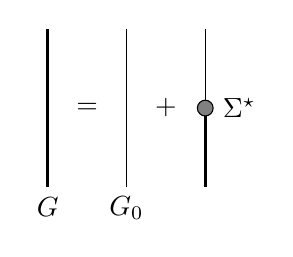
\begin{tikzpicture}[domain=0:4,samples=400]
	\draw[very thick] (0,1) -- (0,-1) node[below] {$G$};
	\node at (0.5,0) {$=$};
	\draw (1,1) -- (1,-1) node[below] {$G_0$};
	\node at (1.5,0) {$+$};
	\draw (2,1) -- (2,0);
	
	\draw[very thick] (2,0) -- (2,-1);
	\draw[fill=gray] (2,0) circle (0.1);
	\node[right] at (2.1,0) {$\Sigma^\star$};
	\end{tikzpicture}
	\caption{Graphic representation of Dyson equation.}
\end{figure}
\begin{thebibliography}{50}
	%\addcontentsline{toc}{chapter}{Bibliography}
	\bibitem{boffi}
	Boffi, S.
	\textit{Da Heisenberg a Landau, un'introduzione alla fisica dei sistemi a molte particelle},
	Bibliopolis,
	2004.
	
	\bibitem{gila}
	Gilardi, G.
	\textit{Analisi Tre},
	McGraw-Hill,
	1994.	
	
	
	
\end{thebibliography}






\end{document}